\chapter{44neV parxkaraNa}

\begin{center}
{\large\bf dashAMsha saMkeSxVpa guNAkArada riVti.}
\end{center}

\begin{verse}
kaM|| matotxMdacacxri riVtiyu| ititxhudada keVLu guMNayx guNakadoLelalxM|| tetitxsutiralaMshagaLava| kitutxta mitavAgi bapapxvututxmamAgaRM||

vi|| guMNayx guNakagaLalilx hecAcxgi dashAMsha sathxLagaLidadxre avugaLalilx eSuTx beVkoV aSuTx dashAMgaLu labadhxdalilx baruva hAge guNisatakakx inonxMdu AshacxrayxvAda riVti uMTu.
\end{verse}

\begin{center}
{\bf\large sUtarx.}
\end{center}

\begin{verse}
kaM|| irabeVkAda dashAMshada | sariyAgeNisutatx guNayx biMduviniMdaM||
barikiVLe guNaka pUNaRdoLiru veVka sAthxnadaMkiyuLiduda balakaM||

$(2)$ taruta dashAMshaMkigaLanu| baribiMduviniMdaviDidu yaDagaDe gAgaM|| diruva guNUNxyXMki mikukxda| paritayxjisuta muMde peVLavxriVtiyanaridaM||

$(3)$ guNaka parxthamAMki meVliha| gaNitada baladaMki modalu guNisutatxdakaM|| deNisuta dashakavanu muMdadhx| vaNisi peVLuva karxmadi guNisi guNisuta poVgu||

$(4)$ muMdeyu guNisuta samayado| LoMdoMdaMshAMki biDuta guNisutalApari|| yiMda bala\-kaMki biDadele| hoMdisi baradavanu kUDi biMduva niVDeY

vi|| labadhxdalilx dashAMsha sathxLagaLu eSuTx irabeVkoV aSuTx aMkigaLanunx guMNAyxMkiya dashAMsha aMkigaLalilx iTuTxkoMDu, A koneV dashAMsha aMkiya keLage guNakada pUNARMkigaLalilxruva EkasAthxnada aMkiyanunx baradukoMDu, uLida pUNARMkigaLanunx balagaDegU, dashAMsha aMkigaLanunx eDagaDegU baradukoLaLxbeVku. A meVle guNakada parxthamAMkiya meVliruva aMkiya bala pAshavxRda aMkiyanunx guNisi, adakekx mAtarx muMde vivarisuva parxkArakekx dashaMkiyanunx tegadukoMDu uLidavugaLanelAlx pUNARMkiya guNAkArada hAgeV guNisi baradukoLaLxbeVku. A meVle aMshagaLalilx oMdoMdaMkiyanunx biTuTx biTuTx adeV parxkArakekx guNisi bariyuvAgeyx balakekx aMki\-yanunx biDada hAge baradu A paMknitxgaLanunx sheVrisi baruva labadhxdalilx koVridaSuTx dashAMsha sathxLadaMki\-yanunx biTuTx biMduvanunx mADabeVku.
\end{verse}

\begin{center}
{\Large\bf idaralilx hiDiya takakx dashakagaLa}\\
\vskip .2cm
{\large\bf karxmavu hAyxgeMdare.}
\vskip .2cm
{\bf\large sUtarx.}
\end{center}

\begin{verse}
kaM|| barutiha guNakoVpariyali| irutiha guNoNxyXMki balada aMkiya guNisa|| labxrutiha dashakada riVtiya| norevenu keVLaduve janake paramAshacxrayxM||

kaM|| sharaviDidu manuvinorigaM| varadashaka dUrxpa keVLu pakaSxdi modalA||
geraDu dashakavanu niVtiLi| sarigakaRdavxyadatanaka gaNitANaRvadoVLf||

kaM|| ipapxtetxYdanu viDidaM| mupapxtutxnAlakxkekx mUru tatapxrakelalxM|| apupxdu patatxdhikakukxM| tapapxde nAlekxYdu I pariyiMdaM||
\end{verse}


\begin{tabular}{>{$}l<{$}>{$}l<{$}>{$}l<{$}>{$}l<{$}}
\text{vi||} & 5\text{riMda} & 14\text{ra varige} & 1\text{deshagi} \\
& 15\text{riMda} & 24\text{ra varige} & 2\text{dashagi}\\
& 25\text{riMda} & 34\text{ra varige} & 3\text{dashagi}\\
& 35\text{riMda} & 44\text{ra varige} & 4\text{dashagi}
\end{tabular}\\

I parxkArakekx $45$ riMda $54$ravarige $5$ dashagiyanUnx muMde $10$ saMKayxgaLu sheVrutAtx hoVgalAgi adakekx oMdoMdu dashakavanunx hecicxsi koLuLxtAtx hoVga beVku.

udAharaNeyu, $23.5678+2`34$ guNAkAra labadhxdalilx $3$ dashAMshagaLu baruva hAge guNisu.\\

\begin{figure}[h]
\centering
\includegraphics[scale=1.3]{2.eps}
\end{figure}

idaralilx dashAMsha sathxLagaLu $3$ sAkeMdu heVLiruvadadxriMda aSuTx dashAMshagaLanunx aMdare, $567$ ravarige iTuTx koMDu muMdina $8$nunx biTuTx biTiTxrutatxde. A meVle, A $7$ra keLage guNakada pUNARMkiyalilx EkasAthxnavAgiruva $2$nunx baradu koMDirutatxde. inunx pUNaRMkigaLu ilalxdadxriMda balakekx aMkigaLanunx bariyalilalxvu. uLida\break apUNARMkiyalilxruva $3$nUnx A meVle $4$nUnx eDagaDege baradukoMDirutatxde.

Agalu $2$riMda $8$nunx guNisalu $16$ idakekx Aguvada dashagiyu $2$ idanunx $2$riMda $7$nunx guNisidadxralilx sheVrisikoMDu muMdakekx sAdhAraNavAgi guNisi bariyalAgi $47136$ Ayitu. A meVle meVlina $7$nunx adara keLagina $2$nUnx biTuTx biTeTxvu.

Iga $3$riMda guNisa beVkAdadxkekx pArxraMBisi $3$riMda $7$nunx guNisalu $21$ idakekx Aguva dashagiyu $2$ idanunx $3$riMda $6$nunx guNisidadxralilx sheVrisikoMDu muMdakekx sAdhAraNavAgi guNisalu $7070$ idanunx eraDaneV sAlinalilx baradirutatxde.

taruvAya meVlina $6$nunx adara keLagina $3$nunx biTuTx biTeTxvu. Iga $4$riMda guNisuvadakekx pArxraMBisi $4$riMda $6$nunx guNisalu $24$, idakekx Aguva dashagi $2$ idanunx $4$riMda $5$nunx guNisidadxralilx sheVrisi koMDu muMdakekx meVlinaMteyeV guNisalAgi $942$ Ayitu, idanunx mUraneV sAlinalilx baradirutatxde. Iga A mUru sAlanUnx kUDisalu $55148$ Ayitu. idaralilx beVkAda dashAMsha sathxlagaLu $3$ AdadxriMda $3$ aMkigaLanunx biTuTx biMduvanunx mADalAgi $55.148$ iSuTx labadhxvAyitu.

\newpage

\begin{center}
{\bf\large tALeyu.}
\end{center}

\begin{figure}[h]
\centering
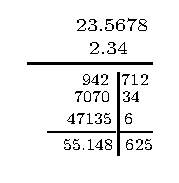
\includegraphics[scale=1.3]{4.eps}
\end{figure}


idaralilx baMdiratakakx $.1486652$ eMbuva $6$ dashAMsha sathxLagaLu bara beVkAdadadxkekx koVrikeV parxkArakekx $148$ eMba $3$ sathxLagaLu mAtarxveV meVlina leKaKxdalilx baMdirutatxde.

\bigskip

\begin{center}
{\bf\Large 60neV aBayx udAraharaNe.}
\end{center}

\begin{enumerate}[\rm(1)]
\item $27.14986\times92.41035$ idanunx $4$ dashAMsha satxLagaLu baruva hAge guNisu.

\item $480.14936\times272416$ idaralUlx dashAMsha satxLagaLu $3$ bara beVku.

\item $1527.310542\times532.78345201$ idaralilx dashAMsha satxLa $5$ sAku.

\item $1\dfrac{3}{4}+\dfrac{7}{8}\times.3456$ idaralilx dashAMsha satxLagaLu $3$ sAku.

\item $45\dfrac{3}{25}+\dfrac{44}{55}-\dfrac{1}{4}$ idanunx $.00078$riMda guNisu dashAMsha satxLa $4$ sAku.
\end{enumerate}



